\documentclass[/Users/ikedahajime/GitHub/reserch/master_report/thesis]{subfiles}
% このファイル内だけのコマンド
\begin{document}
\chapter{手法と数値計算設定}
この章ではシミュレーションの設定と、計測したパラメータについて記す。
\section{数値シミュレーションの設定}
% \cite{filyAthermalPhaseSeparation2012}
\secref{sec:result_abp}では inertial inertial Active Brownian Particles(iABP) モデルを用いた。
iABP モデルは以下のように表される。
% ABPの方程式
\begin{eqnarray}\label{eq:eom_iabp_1}
    m\dot{\bm{v}_i}(t)&=& - \zeta \bm{v}_i  +\bm{F}_i +\zeta v_0 \bm{e}(\theta_i(t))
    % \dot{\bm{r}_i}(t) &=& \zeta \bm{F}_i(t)+v_0 \bm{e}(\theta_i (t))
\end{eqnarray}
\begin{eqnarray}\label{eq:eom_iabp_2}
    \dot{\theta_i }(t) &=& \sqrt{\frac{2}{\tau_p}}\eta_i(t)
\end{eqnarray}
ここで、\mbox{\boldmath$r$}は粒子の位置、$v_0$ は自己推進の速度、$\zeta$ は摩擦係数を表す。
$\eta_i$ はホワイトノイズで、$\langle \eta_i(t) \eta_j(t') \rangle=\delta_{ij}\delta(t-t')$の関係を満たす。
ここで、$\langle \dots \rangle$ はアンサンブル平均である。
$\mbox{\boldmath$e$}(\theta_i)=(\cos\theta_i,\sin \theta_i)$は自己推進の方向を表す単位ベクトルで、
$\tau_p$は持続時間である。
このモデルには2つの緩和時間が存在する。1つは ABP の持つ自己推進の方向を変えるまでの時間であり、
$\tau_p$である。もう1つは慣性による緩和時間であり、これは$\tau_m=m/\zeta$と表される。


$\bm{F}_i$は相互作用を表し、二体間相互作用ポテンシャル$U(r)$と壁との相互作用$\bm{F}_{wall}$を用いて
$\bm{F}_i=-\sum_{i\neq j} \bm{\nabla}_iU(r_{ij})+c_{wall}\bm{F}_{wall}$と書ける。$c_{wall}$は壁による
力の大きさを表す定数で、ここでは1にとった。
ポテンシャルには、Weeks-Chandler-Andersen(WCA)ポテンシャル\cite{weeksRoleRepulsiveForces1971}を用いた。
\begin{equation}
    U(r_{ij})=
    \begin{cases}
        4\epsilon\left(\left(\frac{\sigma}{r_{ij}}\right)^{12}-\left(\frac{\sigma}{r_{ij}}\right)^6+\frac{1}{4}\right) & (r_{ij}<2^{\frac{1}{6}}\sigma)\\
        0 &(r_{ij}>2^{\frac{1}{6}}\sigma)
    \end{cases}
\end{equation}
ここで、$r_{ij}=\left|\bm{r}_i-\bm{r}_j\right|$は粒子間距離、$\sigma$は粒径、$\epsilon$は相互作用の強度である。
\secref{sec:result_abp}では粒子を閉じ込める壁を\figref{fig:setup_circles}(a)のように取る。壁との相互作用には同じポテンシャルを用い、壁による力は
$\bm{F}_{wall}=-\bm{\nabla}U(r_{wall})$と表される。
$r_{wall}$は壁と粒子の距離を表し、$\bm{r}_c$を円の中心をさすベクトルとして$r_{wall}=R+0.5\sigma-\left|\bm{r}-\bm{r}_c\right|$
と表される。

\secref{sec:res_abp_twowall}においては、\figref{fig:setup_circles}(b) のように2つの円をつなげた形の
壁で粒子を閉じ込める。
この系における壁との相互作用についても同様に WCA ポテンシャルを用いた。
$\bm{r}_{c_1}$を$x<0$に存在する粒子が相互作用する円の中心を、
$\bm{r}_{c_2}$を$x>0$に存在する粒子が相互作用する円の中心を指すベクトルとおく。
これらの2つの円の間の距離は$\Delta$であり、2つの円の中心をさすベクトル$\bm{r}_{c_1}、\bm{r}_{c_1}$は
それぞれ$(-\Delta/2,0)、(\Delta/2,0)$と表される。
$r_{wall}$は$r_{wall}=R+0.5\sigma-\left|\bm{r}-\bm{r}_{c_i}\right|$
のようにおいた。ただし、2つの円の接合部である$-0.5\sigma<x<0.5\sigma$においては仮想粒子を$(x,y)=(0,\pm\sqrt{(R+0.5\sigma)^2-(\Delta/2)^2})$
に置いて、それらとの相互作用を壁との相互作用とした。


\begin{figure}
    \centering
    \begin{tabular}{c}
        \begin{minipage}{0.2\hsize}
            \text{(a)}
            \includegraphics[width=\textwidth]{img/method/fig_sincer.png}
        \end{minipage}
        \begin{minipage}{0.35\hsize}
            \text{(b)}
            \includegraphics[width=\textwidth]{img/method/fig_twocer.png}
        \end{minipage}
    \end{tabular}
    \caption[fig:circle]
    {
        (a) 円が1つの系における壁に関する模式図。
        (b) 円が2つの系における壁に関する模式図。
    }
    \label{fig:setup_circles}
\end{figure}
数値計算のため、長さの単位を$\sigma$、時間の単位を$\sigma/v_0$と置いた。無次元化した質量$M=mv_0/\zeta\sigma$、
 Péclet 数$Pe=v_0\tau_p/\sigma$、エネルギーと速度の比$\epsilon^*=\epsilon/\sigma v_0 \zeta$
をパラメータに取り、このうち$\epsilon^*=1$とした。
粒子数$N$は、面積分率$\varphi$と系の面積$S$を用いて$N=4\varphi S/\pi\sigma^2$とした。
コントロールパラメータとして、系の半径$R、Pe、M、\varphi$を用いた。


% コントロールパラメータは、
\secref{sec:result_cabp}では、ABPにキラリティーに関する項を加えた、 Chiral Active Brownian Particles(CABP)%\cite{teeffelenDynamicsBrownianCircle2008}%TODO::aliment forceがないものに変える
を用いた。このモデルは以下のように表される。
% CABPの方程式
\begin{eqnarray}\label{eq:eom_CABP_1}
    \dot{\bm{r}_i}(t) &=& \frac{1}{\zeta} \bm{F}_i(t)+v_0 \bm{e}(\theta_i (t))
\end{eqnarray}
\begin{eqnarray}\label{eq:eom_CABP_2}
    \dot{\theta_i }(t) &=& \Omega+\sqrt{\frac{2}{\tau_p}}\eta_i(t)
\end{eqnarray}
ここで、$\Omega$はキラリティーの強度である。このモデルは ABP にキラリティーの効果を加えたモデルである。
この効果によって粒子の運動方向が曲がり、典型的には円軌道を描く。
その円軌道の半径は$R_\Omega=v_0/\Omega$で表される長さである。
\begin{figure}
    \centering
    \begin{tabular}{c}
        \begin{minipage}{0.6\hsize}
            % \text{(a)}
            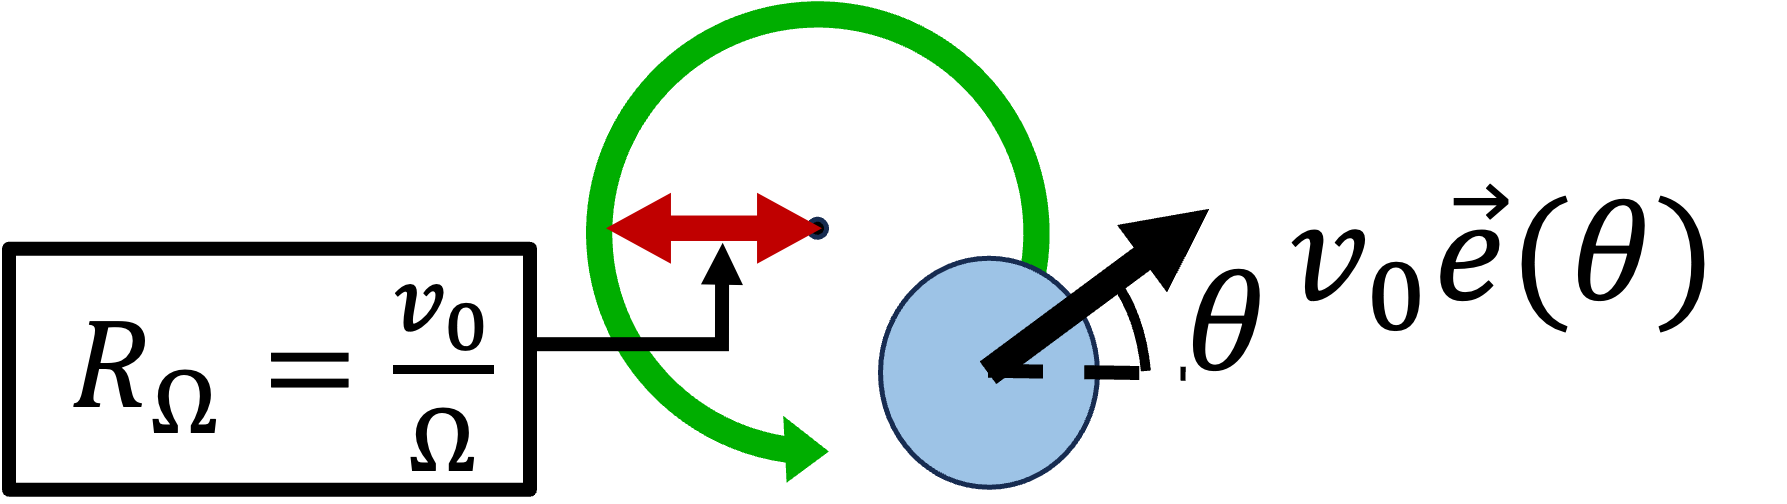
\includegraphics[width=\textwidth]{img/method/cabp_motion.png}
        \end{minipage}
    \end{tabular}
    \caption[Four sample images]
    {
        CABP における運動の模式図。
    }
    \label{fig:sample_four_images}
\end{figure}

ポテンシャルにはHarmonicポテンシャルを用いた。
\begin{equation}
    U(r_{ij})=
    \begin{cases}
        \frac{\epsilon}{2}\left(\frac{r_{ij}}{\sigma}-1\right)^2 &(r_{ij}<\sigma)\\
        0 & (r_{ij}>\sigma)

    \end{cases}
\end{equation}
壁との相互作用には同様にHarmonicポテンシャルを用い、粒子が円の外に出ることを防ぐため、
力の大きさを表す定数を$c_{wall}=100$とした。


本研究では最も簡単な場合として揺らぎがゼロ、つまり持続時間$\tau_p=\infty$の極限を解析した。
$\epsilon^*=40$に固定し、コントロールパラメータとして系の半径$R$、粒子の回転半径$R_\Omega=v_0/\Omega$、面積分率$\varphi$を用いた。


\section{オーダーパラメータ}
観測するパラメータとして、以下のパラメータを用いた。
\subsection{渦秩序変数}\label{subsec:vortes_order_parameter}
系が渦をなしているかどうかを定量化するために、
渦秩序変数$\psi$\cite{wiolandConfinementStabilizesBacterial2013}を以下のように定義する。
\begin{equation}\label{eq:def_psi}
    \psi=\frac{\sum_i \left|\bm{v}_i\cdot \bm{t}_i \right|/\sum_i v_i -2/\pi}{1-2/\pi}
\end{equation}
ここで、$\bm{t}_i$は角度方向の単位ベクトルである。$\psi>0$の時は角度方向の流れが、$\psi<0$の時は動系方向の流れが生じていることがわかる。
特に$\psi\simeq1$の時全ての粒子が角度方向に運動していることを、$\psi\simeq0$の時無秩序な流れが生じていることを示す。


\subsection{規格化された角運動量}
本研究では高密度系でのシミュレーションを行う。この場合、粒子は動径方向の運動をほとんど行わず、角度方向の
運動が支配的になる。そのため\subsecref{subsec:vortes_order_parameter}で定義した渦秩序変数のように
動径方向の運動を考慮したオーダーパラメータを使う必要がない。また、渦秩序変数は渦の回転方向に関する情報を得ることができない。
そこで、以下のように定義される規格化された角運動量$V$\cite{jiangEmergenceCollectiveDynamical2017,capriniCollectiveEffectsConfined2021}を用いる。
\begin{equation}
    V=\frac{1}{N} \sum_i \frac{L_{zi}}{ |L_{zi}|}
\end{equation}
ここで、$L_{zi}$は$i$番目の粒子の角運動量で、$L_{zi}=x_i*v_{yi}-y_i*v_{xi}$。


このパラメータは、角度方向の運動方向が揃っているか、及びその回転方向がどちらかを判定するパラメータである。
まず絶対値に注目すると、絶対値が小さいとき、つまり$|V|\simeq 0$のとき、時計回り、反時計回りに運動する粒子が同数存在し、
系全体での渦が生じていないことが分かる。
反対に絶対値が大きいとき、つまり$|V|\simeq 1$のときは系全体が原点を中心とした一つの渦をなして一方向に回っていることが分かる。


続いて、$|V|\simeq 1$として、その正負について考える。すると、値が負、つまり$V\simeq -1$のときは時計回りの渦が、
値が正、つまり$V\simeq 1$のときは反時計回りの渦が発生していることを読み取ることができる。

\subsection{自己相関関数のフーリエ変換}
\secref{sec:result_abp}では、高密度系において時間に周期性のようなものが見られた。
時間における周期性の判別には、自己相関関数のフーリエ変換がよく用いられる。
まず、速度における時間のフーリエ変換は以下のように定義される。
\begin{equation}
    \tilde{v}(\omega) =\int_{-\infty}^{\infty} dt v(t)e^{-i\omega t}
\end{equation}
ここで、$\omega$は周波数である。
フーリエ変換は、元の関数を様々な周波数を持つ波の重ね合わせとして表現する。この変換後の量$\tilde{v}(\omega)$
は波の持つ振幅を表し、その絶対値$\left|\tilde{v}\right|^2(\omega)$は周波数$\omega$の波が持つエネルギースペクトルを表す。
続いて、自己相関関数のフーリエ変換を考える。
まず、速度の自己相関関数は以下のように表される。
\begin{equation}
    C_v(t)=\int_{-\infty}^{\infty} dt^\prime v(t+t^\prime)v(t^\prime)
\end{equation}
この関数のフーリエ変換は以下のように表される。
\begin{align}
    \tilde{C_v}(\omega)&= \int_{-\infty}^{\infty} dt C_v(t)e^{-i\omega t}\\
    &=\int_{-\infty}^{\infty} dt \left(\int_{-\infty}^{\infty} dt^\prime v(t+t^\prime)v(t^\prime)\right)e^{-i\omega t} \\
    &=\int_{-\infty}^{\infty} dt \int_{-\infty}^{\infty} dt^\prime v(t)v(t^\prime)e^{-i\omega(t-t^\prime)}\\
    &=\int_{-\infty}^{\infty} dt v(t)e^{-i\omega t}\int_{-\infty}^{\infty}dt^\prime v(t^\prime)e^{i\omega t}\\
    &=\tilde{v}(\omega)\tilde{v}^*(\omega)\\
    &=\left| \tilde{v}(\omega) \right|^2
\end{align}
となり、これは速度をフーリエ変換したものの2乗であることがわかる。

この変数の典型的な動きを知るために、相互作用のない一粒子 iABP について解析的に計算する。\equref{eq:eom_iabp_1}、\equref{eq:eom_iabp_2}から、
一粒子 iABP は以下のように表される。
\begin{eqnarray}\label{eq:eom_iabp_single_1}
    m\dot{\bm{v}_i}(t)&=& - \zeta \bm{v}_i  +\zeta v_0 \bm{e}(\theta_i(t))
\end{eqnarray}
\begin{eqnarray}
    \dot{\theta_i }(t) &=& \sqrt{\frac{2}{\tau_p}}\eta_i(t)
\end{eqnarray}
\equref{eq:eom_iabp_single_1}を時間についてフーリエ変換して自己駆動項を$f(t)=v_0 \bm{e}(\theta_i(t))$とおくと、
\begin{eqnarray}
    im\omega\bm{v}&=&- \zeta \bm{v}_i  +\zeta \bm{f}(\omega)
\end{eqnarray}
\begin{eqnarray}
    \bm{v}&=&\frac{\zeta \bm{f}(\omega)}{im+\zeta}
\end{eqnarray}
したがって、
\begin{eqnarray}
    \left|\bm{v}\right|^2&=&\frac{|\bm{f}(\omega)|^2}{\left(1+m^2/\zeta^2\right)}
\end{eqnarray}
ここで、 ABP 系において角度$\theta(t)$の確率分布関数$P(\theta,t)$は
\begin{eqnarray}
    P(\theta,t)&=&\frac{1}{\sqrt{4\pi t/\tau_p}}\exp\left(-\frac{(\theta-\theta_0)^2}{4t/\tau_p}\right)
\end{eqnarray}
である。よって、
\begin{eqnarray}
    \langle f(t)f(0) \rangle&=&\int_{-\infty}^{\infty} d\theta \cos(\theta)P(\theta,t)=e^{-\frac{t}{\tau_p}}
\end{eqnarray}
となるので、一粒子 iABP はに対する速度相関関数のフーリエ変換は以下のように表される。
\begin{equation}\label{eq:intro_ft_about_iabp}
    \left|\bm{v}\right|^2=\frac{|\bm{f}(\omega)|^2}{\left(1+\tau_m^2\right)\left(1+\tau_p^2\right)}
\end{equation}
ここで、$\tau_m=m/\zeta$は慣性の効果による緩和時間である。

この関数の極限について考える。この関数には$\tau_p$と$\tau_m$について対称性が存在する。
そのため、$\tau_p>\tau_m$の場合を考えたとしても関数の性質には影響しないので、ここでは$\tau_p \gg  \tau_m$の場合について考える。
まず$\omega\ll 2\pi/\tau_p$の極限においては$\left|\bm{v}\right|^2 \thicksim v_0^2$であり定数となる。
続いて$2\pi/\tau_p \leq \omega \leq 2\pi/\tau_m$の領域では、$\left(1+\tau_m^2\right)$の項が無視できるほど小さいため
この関数は$\omega^{-2}$に比例する。その後$\omega \gg 2\pi/\tau_m$においては$\omega^{-4}$に比例する。

\begin{figure}
    \centering
    \begin{tabular}{c}
        \begin{minipage}{0.7\hsize}
            % \text{(a)}
            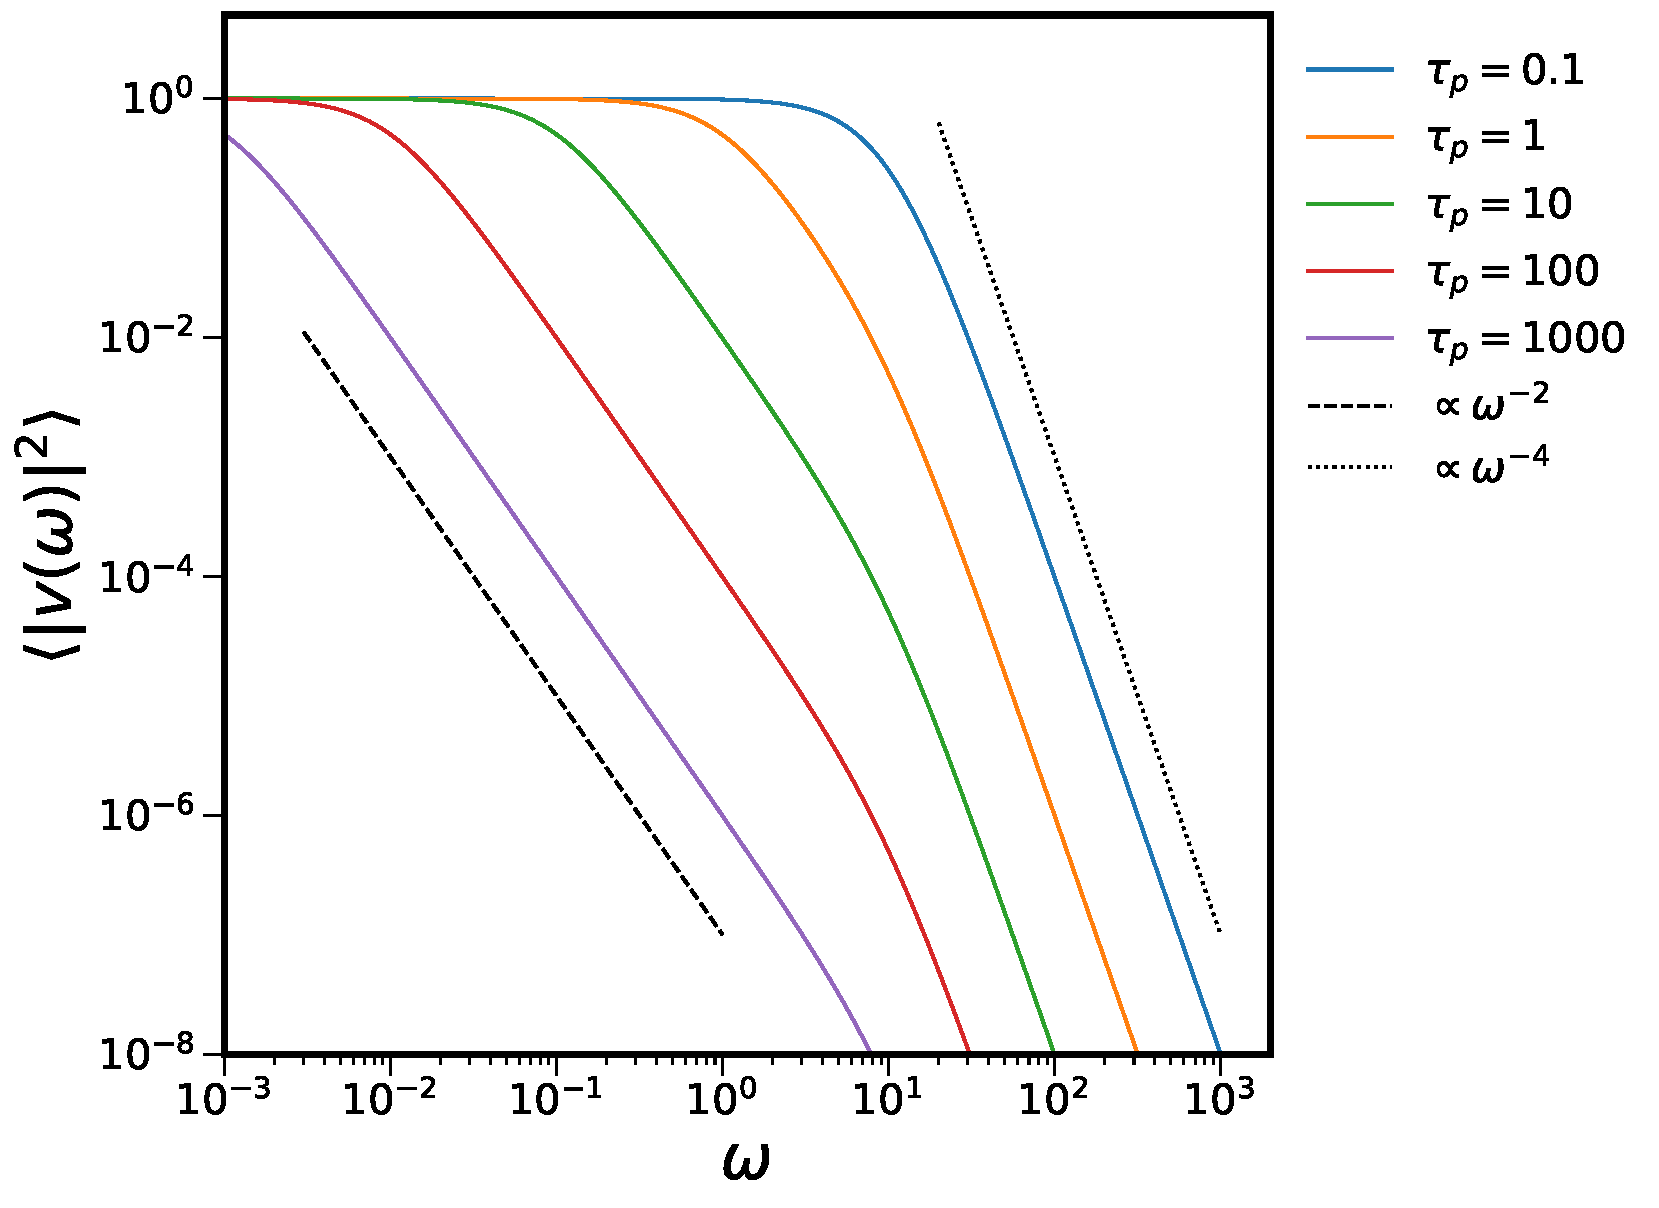
\includegraphics[width=\textwidth]{img/method/ft_vcor.pdf}
        \end{minipage}
    \end{tabular}
    \caption[Four sample images]
    {
        一粒子 iABP における速度の自己相関関数のフーリエ変換の理論曲線。
        $\tau_{m}=0.1$に固定した。図中の曲線は、それぞれ異なる$\tau_p$におけるグラフを表し、
        点線はそれぞれ$\omega^{-2}、\omega^{-4}$に比例する直線を表す。
    }%TODOレーヴェンのcabp len ni
    \label{fig:method_ft_single}
\end{figure}


この結果をグラフにしたものが\figref{fig:method_ft_single}である。
この図からも分かるように、2つの緩和時間$\tau_m$と$\tau_p$の大小によって
グラフはその冪を変える。
%TODO:一粒子系のず

\subsection{円を2つに分けた時の物理量}
粒子を拘束する円を2つに分けた時の物理量は渦秩序変数、および規格化された角運動量を円が2つの場合に拡張したものを使う。
このオーダーパラメータは以下のように定義される。
\begin{equation}
    V_2={\mathop{\mathrm{sign}}\nolimits} (V)\sqrt{|V|}
\end{equation}
ここで、$V=(\sum_{x<0} L_{zc_1}/|L_{zc_1}|)(\sum_{x>0}L_{zc_2}/|L_{zc_2}|)$で、$L_{zc_i}$は$r_{c_i}$を中心とする角運動量である。
このパラメータは、渦が強磁性的で2つの渦が同じ方向に渦巻いているのであれば1を、
反強磁性的2つの渦が逆の方向に渦巻いているのであれば-1にそれぞれ近づくことを表す。
また、この系における渦秩序変数を以下のように定義する。
\begin{equation}
    \varphi_2=\frac{(\sum_{x<0} \left|\bm{v}\cdot \bm{t}_{1} \right|+\sum_{x>0} \left|\bm{v}\cdot \bm{t}_{2} \right|)/\sum_i v_i -2/\pi}{1-2/\pi}
\end{equation}
ここで、$\bm{t}_1、\bm{t}_2$は、それぞれ左、右の円における壁に並行な単位ベクトル。
この変数は円が1つの場合の渦秩序変数と同じことを表す。つまり、$\psi>0$の時は角度方向の流れが、$\psi<0$の時は動系方向の流れが生じていることがわかる。
特に$\psi\simeq1$の時全ての粒子が角度方向に運動していることを、$\psi\simeq0$の時無秩序な流れが生じていることを示す。




\subsection{渦度}\label{subsec:def_vortex}
渦度場は、速度場$\bm{v}(\bm{r})$を用いて$\omega(\bm{r})=\partial_x v_y -\partial_y v_x$と表される。
数値計算上、速度場は以下のように計算する。空間を$\delta x=\delta y=0.25 \sigma$の格子状に分割する。
このとき、格子点$r(i,j)$における速度場は%この書き方でいいのか?
\begin{equation}\label{eq:valocity_field}
    \bm{v}(r(i,j))=\sum_{\left|\bm{r}_k-r(i,j)\right|<3\sigma} f(\left|\bm{r}_k-r(i,j)\right|)\bm{v}_k
\end{equation}
のように計算する。ここで、$f(r)=(2\pi s^2)^{-1} \exp(-r^2/2s^2)$はガウシアン関数であり、分散$s$は$3/\sqrt{2\log 10}$とした。


この速度場を用いて、渦度場は格子点の周りの速度場を線積分することで計算される。
\begin{equation}
    \omega (r(i,j))=\frac{v_x(r(i,j))\delta x +v_y(r(i+1,j)) \delta y -v_x(r(i+1,j+1))\delta x -v_y(r(i,j+1))}{\delta x \delta y}
\end{equation}

\subsection{方位角成分の運動量}
円の中に生じる渦の定量化のため、方位角成分の運動量を導入する\cite{nishiguchiVortexReversalPrecursor2024}。
この量は円の中に複数の渦があることを示す量であり、$m_n$は$2n$個の渦があることを表す。
方位角成分の運動量は以下のように定義される。
\begin{eqnarray}
    m_n &=& \int_0^R dr r\left|\frac{1}{2\pi}\int_0^{2\pi}d\theta \bm{v}(r,\theta)\right|^2
\end{eqnarray}
ここで、$\bm{v}(r,\theta)$は極座標系の速度場である。
数値計算する際には、\subsecref{subsec:def_vortex}と同様に式\equref{eq:valocity_field}に基づいて求めた速度場を使用し、
積分計算には幅0.25の中点法を用いた。
ただし、ここで用いる速度場では格子点を$x$軸、$y$軸共に格子の半分$\delta x/2=\delta y/2=0.125$だけ平行移動して計算した。

\subsection{結晶秩序変数}
結晶化について議論するためのオーダーパラメータの1つに結晶秩序変数$\phi_6$がある。
このパラメータは系が結晶構造をなしているかを表す物理量である。
本研究では、以下のように定義される、一粒子に対するパラメータ$\phi_{6j}$を用いる。
\begin{equation}
    \phi_{6j}=\frac{1}{6}\sum_{k\in \mathcal{N}_{6j}} e^{6i\theta_{jk}}
\end{equation}
ここで、$\mathcal{N}_{6j}$は$j$番目の粒子の6つの最近接粒子を、$\theta_{jk}$は
ベクトル$\bm{r}_j-\bm{r}_k$がx軸となす角度である。
% TODO:もっと説明
\end{document}
